% created on 2019-12-13
% @author : bmazoyer

%% Lines to compile only this capter
\documentclass[11pt, twoside, a4paper, openright]{report}
\usepackage[utf8]{inputenc}
% \DeclareUnicodeCharacter{223C}{~}

%Bibliography style
% \usepackage[square, numbers]{natbib}
% \usepackage[round]{natbib}
% \usepackage{biblatex}
% \bibliographystyle{unsrtnat}
% \bibliographystyle{unsrt}
% \bibliographystyle{plain}
% \bibliographystyle{aa}
% \usepackage[backend=bibtex,style=authoryear,natbib=true]{biblatex} 
\usepackage[
backend=biber,
style=authoryear,
citestyle=authoryear,
url=false
]{biblatex}
\addbibresource{../source/library.bib}

\usepackage[T1]{fontenc}
\usepackage[french]{babel}
\usepackage{csquotes}  % used for citations (recommended when using biblatex)
%\usepackage{helvet}
%\renewcommand{\familydefault}{\sfdefault}
\usepackage{mathptmx}
\usepackage{amssymb}
\usepackage{geometry} 
\usepackage{xcolor}
\usepackage[absolute,overlay]{textpos}
\usepackage{graphicx}
\usepackage{lipsum}
\usepackage[explicit]{titlesec}
\usepackage{lmodern}
\usepackage{color}
\usepackage{array}
\usepackage{mathtools}
\usepackage{caption}
\usepackage{multicol}
\usepackage{booktabs}
\usepackage{enumitem}
\usepackage{hyperref}
\usepackage{afterpage}
\usepackage{emptypage}
\usepackage{setspace}
\usepackage{pgffor}
    \setlength{\columnseprule}{0pt}
    \setlength\columnsep{10pt}
\usepackage[francais,nohints]{minitoc}
    \setcounter{minitocdepth}{3}
 
 %https://la-bibliotex.fr/2019/02/03/ecrire-les-nombres-et-les-unites-avec-latex/   
\usepackage{siunitx}
% \sisetup{
%     detect-all,
%      output-decimal-marker={,},
%      group-minimum-digits = 3,
%      group-separator={~},
%      number-unit-separator={~},
%      inter-unit-product={~},
%      list-separator = {, },
%      list-final-separator = { et },
%      range-phrase = --,
%      separate-uncertainty = true,
%      multi-part-units = single,
%      list-units = single,
%      range-units = single
%     }
\usepackage{physics}
\usepackage{isotope}

\usepackage[perpage]{footmisc} % to reset the counter of footnote each page

    
\usepackage{fancyhdr}			% Entête et pieds de page. Doit être placé APRES geometry
\pagestyle{fancy}		% Indique que le style de la page sera justement fancy
%\lfoot[\thepage]{} 		% gauche du pied de page
%\cfoot{} 			% milieu du pied de page
%\rfoot[]{\thepage} 
\fancyfoot{} % vide le pied~de~page
\fancyfoot[LE,RO]{\thepage}
\fancyfoot[LO,CE]{}% droite du pied de page
\fancyhead{}	
\fancyhead[LE]{\leftmark}	
\fancyhead[RO]{\rightmark}

\fancypagestyle{plain}{%
\fancyhf{} % vide l’en-tête et le pied~de~page.
\fancyfoot[LE,RO]{\thepage} % numéro de la page en cours en gras% et centré en pied~de~page.
\renewcommand{\headrulewidth}{0pt}
\renewcommand{\footrulewidth}{0pt}}



% Premiere page des chapitres
\newlength\chapnumb
\setlength\chapnumb{3cm}
 
\titleformat{\chapter}[block] {
  \normalfont}{}{0pt} { %police
    \parbox[b]{\chapnumb}{
      \fontsize{120}{110}\selectfont\thechapter} %taille du chiffre
      \parbox[b]{\dimexpr\textwidth-\chapnumb\relax}{
        \raggedleft 
        \hfill{\bfseries\Huge#1}\\ %taille du titre
        \rule{\dimexpr\textwidth-\chapnumb\relax}{0.4pt} %ligne de separation
  }
}
 
 %premiere page chapitre non numerote (remerciement, table des matieres ...)
 
\titleformat{name=\chapter,numberless}[block]
{\normalfont}{}{0pt}
{   
    \parbox[b]{\dimexpr\textwidth}{%   
    \hfill{\bfseries\Huge#1}\\
  \rule{\dimexpr\textwidth}{0.4pt}}}
    
 %   \titleformat{name=\chapter,numberless}[block]
%{\normalfont}{}{0pt}
%{\parbox[b]{\chapnumb}{%
%   \mbox{}}%
%  \parbox[b]{\dimexpr\textwidth-\chapnumb\relax}{%
%    \raggedleft%
%    \hfill{\bfseries\Huge#1}\\
%    \rule{\dimexpr\textwidth-\chapnumb\relax}{0.4pt}}}


%%%    SIunitx
\sisetup{locale = FR,
  % inter-unit-product=\ensuremath{\cdot},
  inter-unit-product=\ensuremath{\,},
  per-mode=reciprocal,
  separate-uncertainty = true,
  detect-all
}
\DeclareSIUnit{\Mpc}{Mpc}
\DeclareSIUnit{\kpc}{kpc}
\DeclareSIUnit{\Gpc}{Gpc}
\DeclareSIUnit{\h}{\textit{h}~}
\DeclareSIUnit{\perh}{\textit{h}^{-1}\,}

%%% Geometry
\geometry{
left=20mm,
top=30mm,
right=20mm,
bottom=30mm
}

%%% Color
\definecolor{bordeau}{rgb}{0.3515625,0,0.234375}

%%% Commands
\newcommand{\Nmocks}{\num{30}}
\newcommand{\hMpc}{h^{-1}\,\mathrm{Mpc}}
\newcommand{\hGpc}{h^{-1}\,\mathrm{Gpc}}
\newcommand{\kms}{\mathrm{km\,s^{-1}}}

\newcommand{\lya}{Ly$\alpha$}
\newcommand{\lyb}{Ly$\beta$}
\newcommand{\lyalya}{Ly$\alpha$(Ly$\alpha$)}
\newcommand{\lyalyb}{Ly$\alpha$(Ly$\beta$)}

\newcommand{\lrf}{\lambda_{\rm RF}}
\newcommand{\kpar}{k_{\parallel}}
\newcommand{\apar}{\alpha_{\parallel}}
\newcommand{\rpar}{r_{\parallel}}
\newcommand{\aperp}{\alpha_{\perp}}
\newcommand{\rperp}{r_{\perp}}
\newcommand{\kperp}{k_{\perp}}

\newcommand{\blya}{b_{\rm Ly\alpha}}
\newcommand{\betalya}{\beta_{\rm Ly\alpha}}
\newcommand{\blyb}{b_{\rm Ly\alpha}}
\newcommand{\betalyb}{\beta_{\rm Ly\beta}}
\newcommand{\dlya}{d_{\rm Ly\alpha}}
\newcommand{\bhcd}{b_{\rm HCD}}
\newcommand{\betahcd}{\beta_{\rm HCD}}
\newcommand{\Fhcd}{F_{\rm HCD}}
\newcommand{\Lhcd}{L_{\rm HCD}}

\newcommand{\imin}{i_{\rm min}}
\newcommand{\imax}{i_{\rm max}}
\newcommand{\jmin}{j_{\rm min}}
\newcommand{\jmax}{j_{\rm max}}

\newcommand{\xioned}{\xi_{\rm 1d}}
\newcommand{\DHub}{D_{H}}
\newcommand{\DM}{D_{M}}

\newcommand{\omegam}{\Omega_M}
\newcommand{\omegac}{\Omega_C}
\newcommand{\omegab}{\Omega_B}
\newcommand{\omegan}{\Omega_\nu}
\newcommand{\omegal}{\Omega_\Lambda}
\newcommand{\omegak}{\Omega_k}
\newcommand{\orad}{\Omega_R}
\newcommand{\ogam}{\Omega_\gamma}
\newcommand{\lcdm}{$\Lambda$CDM}

\newcommand{\picca}{\texttt{picca}}

%%% Rem's command
\newcommand\blankpage{%
    \null
    \thispagestyle{empty}%
    \addtocounter{page}{-1}%
    \newpage}
  
% Command to set up a particular alignment for a cell in tabular :
% \myalign{c}{foo} for instance
\newcommand*{\myalign}[2]{\multicolumn{1}{#1}{#2}}
 
\renewcommand{\thesection}{\arabic{section}}

% Romain
\newcommand{\cRM}[1]{\MakeUppercase{\romannumeral #1}}	% Capital
\newcommand{\cRm}[1]{\textsc{\romannumeral #1}}	% Petit majuscule
\newcommand{\crm}[1]{\romannumeral #1}
% Siècle %
\newcommand{\siecle}[1]{\cRm{#1}\textsuperscript{e}~siècle}



% Thesis title
\newcommand{\PhDTitle}{Les forêts \lya{} du relevé eBOSS : comprendre les fonctions de corrélation et les systématiques} 

% Name
\newcommand{\PhDname}{Thomas Etourneau} 

% Change this variable if you add or remove chapters
\newcommand*{\NumOfChapters}{6}

% Change this variable if you add or remove appendices
\newcommand*{\NumOfAppendices}{2}

% PDF metadata
\hypersetup{
	pdfauthor={\PhDname},
	pdfsubject={Manuscrit de thèse de doctorat},
	pdftitle={\PhDTitle}
}


\begin{document}
%%

\graphicspath{ {../figures/mocks/} }

\chapter{Développement des mocks}
\minitoc
\newpage
\thispagestyle{fancy}

\textbf{Dans ce chapitre, nous présentons la construction des \emph{mocks} : des spectres de quasars simulés, dont les forêts \lya{}
sont corrélées entre elles et avec le champ de quasars sous-jacent.
%  et le champ de quasars possèdent les bonnes fonctions d'auto corrélation et de corrélation croisée.
% des simulations qui visent à reproduire les données d'eBOSS et de DESI. Ces mocks, nommés \texttt{SaclayMocks} et présentés dans \citet{CITE:mocks}, sont le c{\oe}ur de ce manuscrit.
Ces mocks visent à reproduire les données d'eBOSS et de DESI. Ils sont nommés \texttt{SaclayMocks} et présentés dans \citet{CITE:mocks}.}
Le code est écrit en Python\footnote{https://www.python.org/} et se trouve en accès libre sur GitHub\footnote{https://github.com/igmhub/SaclayMocks}. L'utilisation de ces mocks et leur validation seront présentés dans les chapitres suivants.

\section{Objectifs des mocks}
% Les mocks s'inscrivent dans le projet DESI, et sont utilisés dans l'analyse finale des données eBOSS \citep{CITE:dr16}.
Contrairement à ce qu'on appelle les simulations, les mocks ne contiennent pas de physique à proprement parler : ils ne sont pas utilisés afin de déduire des paramètres astrophysiques. Certaines simulations, les simulations hydrodynamiques, permettent de mesurer des effets astrophysiques, comme par exemple le biais de l'hydrogêne ou du \lya{}. Mais ces simulations sont très couteuses car elles nécessitent de modéliser les effets physiques qui affectent les paramètres mesurés.
Les mocks, quant à eux, sont conçus afin de répliquer rapidement un jeu de données, dans le but de tester l'analyse qui sera appliquée sur ces données.
% Dans le cas de l'analyse \lya{} d'eBOSS et de DESI, les mocks sont utilisés afin
Les mocks sont donc utilisés afin
\begin{itemize}[label=$\bullet$]
\item de vérifier la mesure des paramètres $\apar{}$, $\aperp{}$ : cette mesure est-elle non biaisée ?
\item d'identifier les potentielles systématiques : la présence de métaux et d'HCD dans les données est-elle bien modélisée ? Affecte-t-elle la mesure de $\apar{}$, $\aperp{}$ ?
\item de tester la matrice de distorsion : la distorsion de la fonction de corrélation due à l'ajustement du continuum du quasar est-elle correctement prise en compte par la matrice de distorsion ?
\item de vérifier l'estimation de la matrice de covariance : la matrice de covariance, calculée à partir des données, est-elle bien estimée ?
\end{itemize}
La production et l'analyse d'un grand nombre de mocks permet de répondre précisément à ces questions. Ces mocks sont donc nécessaires pour pouvoir valider l'analyse menée sur les données.

\paragraph{}
Les mocks décrits dans ce manuscrit s'inscrivent dans les projets eBOSS et DESI. Ils sont utilisés dans l'analyse \lya{} des données complète d'eBOSS \citep{CITE:dr16}, et seront utilisés dans l'analyse \lya{} de DESI.
L'objectif de ces mocks est donc de répliquer au mieux les données \lya{} d'eBOSS et de DESI. Ces relevés couvrent un volume de plusieurs dizaines de \si{\cubic\Gpc}, et les échelles sondées grâce au \lya{} descendent jusqu'à la centaine de \si{\kpc}. Les mocks nécessitent donc de reproduire un volume immense, avec une bonne résolution.
Les simulations dites \emph{N-corps} sont des simulations qui traitent le problème à N corps.
% Elles sont initialisées avec une distribution de matière noire, représentée par des macro-particules de masse $\sim 10^{9} M_{\odot}$, à un redshift élevé ($z > 100$).
\textbf{Elles sont initialisées à un redshift élevé ($z > \num{100}$), avec une distribution de matière noire représentée par des macro-particules. Généralement, environ $(\num{10000})^3$ macro-particules sont présentes dans ces simulations. La masse de ces particules dépend du volume simulé. Par exemple, pour un volume d'environ $(\SI{4}{\Gpc})^3$, les particules possèdent une masse $\sim 10^{9} M_{\odot}$ \citep{Heitmann2019}.}
Puis, à chaque pas de temps, ces macro-particules sont déplacées en considérant uniquement les interactions gravitationnelles. Le champ de matière initial évolue ainsi jusqu'à $z=0$. Ces simulations sont très utiles pour étudier les effets de la gravité à grande échelle. Cependant elles ne sont pas adaptées à notre utilisation : afin d'avoir la résolution et le volume requis, la simulation nécessiterait beaucoup trop de macro-particules pour être réalisable dans un temps raisonnable.

Les simulations hydrodynamiques fonctionnent de la même manière que les simulations N-corps. Elles incluent, en plus des macro-particules de matière noire, la physique baryonique présente dans le milieu galactique. Les baryons sont aussi représentés par des macro-particules. Afin de résoudre l'intérieur des galaxies, les macro-particules utilisées possèdent une masse plus faible que dans le cas des simulations N-corps. En contrepartie, le volume simulé est plus petit. Dans le cas des simulations hydrodynamiques, la densité, la pression et la tempéature sont tracées dans chaque cellule. Certains effets astrophysiques, comme les supernovae ou les AGN peuvent aussi être présents. 
% Cependant, ces simulations ne sont pas non plus adaptées à notre utilisation car le volume d'univers simulé est bien trop petit : quelques dizaines de \si{\perh\cubic\Mpc}.
\textbf{Ces simulations nécessitent encore plus de temps de calcul que les simulations N-corps. Elles ne sont donc pas non plus adaptées à notre utilisation.}

Ainsi, avoir un grand volume et une grande résolution requiert l'utilisation des \emph{champs aléatoires gaussiens} (GRF pour Gaussian Random Field). Ce sont des champs qui en chaque point prennent une valeur aléatoire selon une statistique gaussienne.
Une fois générés, il est possible de donner à ces champs n'importe quelle fonction de corrélation, en utilisant la transformation de Fourier. Les GRF sont donc idéaux pour simuler le champ de matière à grande échelle.
\textbf{Ces champs sont utilisés notament dans les simulations N-corps, afin de fournir les conditions initiales.}
Cependant, l'utilisation des GRF ne donne pas accès aux non linéaritées qui peuvent émerger dans l'évolution des similutaions N-corps et hydrodynamiques. La seule information provient de la fonction de corrélation que l'on applique au GRF.
\textbf{Mais cela est entièrement suffisant pour l'utilisation que nous en avons dans ce manuscrit : nous générons un champ gaussien destiné à simuler le champ d'absorption \lya{} et le champ de quasars, dont les fonctions d'auto corrélation et de corrélation croisée sont choisies afin de correspondre à ce qui est observé dans les données.}


\section{Construction des mocks}
\textbf{Dans cette section, nous détaillons comment les mocks sont générés.
Nous présentons d'abord la génération des champs de densité,
% puis de ces champs de densité, comment sont tirés les quasars.
puis comment les quasars sont tirés à partir de ces champs de densité.
%Nous expliquons ensuite comment, de la position de chaque quasar, nous créons sa ligne de visée.
Nous expliquons ensuite comment nous calculons la densité le long de la ligne de visée de chaque quasar.
% Enfin, nous présentons comment de la densité le long de la ligne de visée nous calculons la fraction de flux transmis et comment nous tirons les HCD.
Enfin, nous présentons comment la densité le long de la ligne de visée est transformée en fraction de flux transmis, et comment nous tirons les HCD.}


\subsection{Les champs de densité}
\label{subsec:densityfields}
La première étape dans la création des mocks est de générer les boîtes qui contiennent le champ de densité $\delta$. D'abord, un GRF est généré dans une boite de $\num{2560}\times\num{2560}\times\num{1536}$ voxcells, chaque voxcell faisant  $d_{cell}^3 = (\SI{2.19}{\perh\Mpc})^3$.
Afin que le champ $\delta$ possède la bonne fonction de corrélation, une transformation de Fourier 3D\footnote{Nous utilisons la librairie pyFFTW (https://github.com/pyFFTW/pyFFTW), une adaptation python de la librairie FFTW (http://www.fftw.org/).} est appliquée sur la boîte, puis la boîte $\delta_k$ ainsi obtenue est multipliée par
\begin{equation}
  \sqrt{\frac{P(k)}{d_{cell}^3}} \; ,
\end{equation}
\textbf{où $P(k)$ est le spectre de puissance désiré. Ce procédé garanti que le champ $\delta_k$ suive le spectre de puissance $P(k)$. Il est ensuite possible d'obtenir la boîte $\delta$ dans l'espace réel grâce à une transformation de Fourier inverse de la boîte $\delta_k$.}

% Le GRF pourrait être tiré directement dans l'espace $k$ mais nous ne perdons pas beaucoup de temps CPU\footnote{Le temps CPU (Central Processing Unit) désigne le temps utilisé par les processeurs d'une machine pour exécuter un code.} à procéder comme cela.
\textbf{Le GRF pourrait être tiré directement dans l'espace $k$. Dans ce cas, il nous faut tirer deux champs gaussiens : un pour la partie réelle, et un autre pour la partie imaginaire. La transformation de Fourier prenant moins de temps que la génération du champ aléatoire, nous préférons générer le champ dans l'espace réel plutôt que dans l'espace $k$.
% Nous distingons ici deux champs : le champ utilisé pour tirer les quasars, et le champ utilisé pour créer l'absorption \lya{}. Ces deux champs requièrent deux spectres de puissance différents, et donc deux boîtes de densité différentes.
Dans la suite nous décrivons les différentes boîtes nécessaires à la construction des mocks : les boîtes champs utilsées pour tirer les quasars, la boîte utilisée pour créer l'absorption \lya{}, ainsi que les boîtes de vitesse et de gradient de vitesse. Afin de garantir leur corrélation, toutes ces boîtes sont construites à partir de la même boîte initial $\delta_k$.}

\subsubsection{Les quasars}
\label{subsubsec:boiteqso}
\textbf{Afin de construire un relevé de quasars corrélés, nous tirons les quasars selon le champ dans l'espace réel $\delta_{\textsc{QSO}}$, construit à partir de $\delta_k$. Une première solution est de tirer les quasars dans les cellules dont le champ $\delta_{\textsc{QSO}}$ est supérieur à un certain seuil. Cette solution produit une fonction de corrélation correcte aux grandes échelles, mais pas aux petites.
En effet, comme expliqué précédemment, l'utilisation des GRF ne permet pas de capturer l'évolution non linéaire du champ de matière, qui se manifeste aux petites échelles.
Plutôt que de modéliser ces non linéarités, nous considérons une seconde solution : nous considérons que les quasars suivent une distribution log-normale. Ceci permet d'obtenir une meilleure corrélation aux petites échelles.
% Comme expliqué précédemment, l'utilisation des GRF ne permet pas de capturer l'évolution non linéaire du champ de matière. Plutôt que de modéliser ces non linéaritées, nous considérons que les quasars suivent une distribution log-normale.
Ce choix est souvent fait pour simuler des relevés de galaxies \citep{agrawal_generating_2017}, et est en accord avec ce qui est observé dans les données \citep{Clerkin2016}.
% Ainsi, au lieu de placer les quasars dans les voxcells qui possèdent une densité plus élevé qu'un certain seuil, nous tirons les quasars dans chaque voxcell avec une probabilité
Ainsi, dans chaque voxcell, les quasars sont tirés avec une probabilité}
\begin{equation}
  P \propto \mathrm{e}^{\delta_q} \; ,
\end{equation}
où $\delta_q$ est le champ de densité dans le voxcell considéré.
Comme montré par \citet{coles_lognormal_1991}, afin que les quasars suivent la fonction de corrélation $\xi(r)$, le champ $\delta_q$ doit suivre la fonction de corrélation 
\begin{equation}
  \label{eq:lognormal}
  \xi_q(r) = \ln(1+\xi(r)) \; .
\end{equation}
Nous verrons section~\ref{subsec:qso} que, de manière à obtenir un relevé synthétique de quasars dont le biais dépend de $z$, nous utilisons trois boîtes qui suivent des distributions log-normales, à des redshifts différents. La probabilité pour tirer les quasars dépend de l'interpolation de ces 3 boîtes.
% Ces champs sont construits aux redshits $z_1 = \num{1.9}$, $z_2 = \num{2.75}$, et $z_3 = \num{3.6}$.
Pour chacune des boîtes, nous partons du spectre de puissance de la matière $P_{matière}(k)$ à $z=0$, fournit par Camb \citep{Lewis1999}. Nous multiplions ensuite ce spectre de puissance par $(b_{\textsc{QSO}}(z_i) G(z_i))^2$, où $i \in [1, 2, 3]$. A l'aide de la transformation de Fourier, nous calculons la fonction de corrélation $\xi_{i}(r)$. Puis, nous déterminons le spectre de puissance $P_{\textsc{QSO},i}(k)$, à appliquer à la boîte $\delta_k$, comme la transformée de Fourier de $\xi_{\textsc{QSO},i}(r) = \ln(1+\xi_i(r))$ (équation~\ref{eq:cf_tf2}).
Une fois les trois spectres de puissances $P_{\textsc{QSO},i}(k)$ obtenus, nous construisons 3 boîtes
\begin{equation}
  \delta_{k,i}(k)  = \delta_k(k) \sqrt{\frac{P_{\textsc{QSO},i}(k)}{V_{cell}}} \; ,
\end{equation}
où $\delta_k$ est le GRF dans l'espace de Fourier. Une fois ces 3 boîtes construites, nous appliquons à chacune d'entre elle une transformation de Fourier inverse afin d'obtenir les boîtes $\delta_{\textsc{QSO}, i}$. Ces boîtes seront interpolées en $z$, puis les quasars seront ensuite tirés avec une probabilité $\propto \exp(\delta_{\textsc{QSO}}(z))$, où $\delta_{\textsc{QSO}}$ est la boîte interpolée. Nous expliquons cette étape dans la section~\ref{subsec:qso}.


\subsubsection{Le champ \lya{}}
Afin de construire le champ d'absorption \lya{}, nous avons besoin du champ de densité de l'hydrogène neutre. Comme expliqué dans la section~\ref{subsec:lya}, la fraction de flux transmis $F$ est reliée à la profondeur obtique $\tau$ par
\begin{equation}
  F = exp(- \tau) \; .
\end{equation}
De plus, la formule FGPA (Fluctuating Gunn Peterson Approximation) permet de relier la profondeur optique $\tau$ au contraste de densité $\delta$ à $z = 0$ :
\begin{equation}
  \label{eq:fgpa1}
  \tau(z) = a(z) \mathrm{e}^{b(z) G(z) \delta} \;
\end{equation}
Les paramètres $a$ et $b$ sont des paramètres à ajuster afin d'obtenir le bon biais du \lya{} et la bonne transmission moyenne $\overline F$. Leur détermination est décrite dans la section~\ref{prov}. Le facteur de croissance $G$ prend en compte l'évolution avec le redshift du champ de densité $\delta$. Ainsi il nous suffit de construire un GRF qui suit la fonction de corrélation à $z=0$ pour simuler le champ d'absorption du \lya{}. Pour ce faire, nous partons de la même boîte $\delta_k$ utilisée pour construire les 3 boîtes log-normales des quasars. Ceci garanti la corrélation croisée entre les quasars et le champ d'absorption \lya{}. Le spectre de puissance de la matière $P_{matière}(k)$ à $z=0$ est ensuite appliqué à la boîte $\delta_k$. Enfin, nous obtenons la boîte de densité $\delta_{matière}$ à $z = 0$ qui servira au calcul du champ d'absorption du \lya{} en effectuant la transformée de Fourier de la boîte
\begin{equation}
  \delta_{k, matière}(\vec k)  = \delta_k(\vec k) \sqrt{\frac{P_{matière}(\vec k)}{V_{cell}}} \; .
\end{equation}


\subsubsection{Les champs des vitesses}
\label{subsubsec:vitesses}
Afin d'inclure les RSD dans nos mocks, nous simulons aussi le champ des vitesses. A l'ordre linéaire, le champ des vitesses $v_{k,n}$ dans l'espace $k$ selon la direction $\vec u_{n}$, avec $n \in [\textsc{x},\textsc{y},\textsc{z}]$, est relié au champ de densité $\delta_k$ par la relation (\#prov mettre la démo ? voir dodelson)
\begin{equation}
  \label{eq:v1}
  v_{k,n}(\vec k) = \frac{ik_n}{k^2} \dot a f \delta_{k}(\vec k) \; .
\end{equation}
% Le champ $\delta_{k, matière}$ est le champ de fluctuation de la matière à $z = 0$ dans l'espace $k$ calculé précédemment.
Il est fréquent (\#prov approximation réaliste ? mettre une source) de considérer que le champ de vitesse des traceurs est le même que celui de la matière sous-jacente. Autrement dit, le champ de vitesse des traceurs est non biaisé.
En ce qui concerne les quasars, nous simulons les RSD en déplaçant chaque quasar proportionnellement à sa vitesse le long de la ligne de visée (équation~\ref{eq:delta_z}). Dans ce but, nous calculons les trois boîtes de vitesses $v_{k,\textsc{x}}$, $v_{k,\textsc{y}}$ et $v_{k,\textsc{z}}$ à $z=0$, comme
\begin{equation}
  v_{k, n}(\vec k) = \frac{- i k_n}{k^2} H_{0} \frac{dG}{dz} \delta_{k, matière}(\vec k) \; ; \hspace{0.5cm} n \in [\textsc{x}, \textsc{y}, \textsc{z}] \; .
\end{equation}
Cette équation est équivalente à l'équation~\ref{eq:v1} pour $z=0$.
Comme précédemment, la boîte $\delta_{k, matière}$ est la même que celle utilisée pour construire les boîtes $\delta_{\textsc{QSO},i}$ des quasars et la boîte $\delta_{matière}$ utilisée pour le \lya{}, ceci afin de garantir la corrélation entre la densité des traceurs et leurs vitesses particulières. A l'aide d'une transformation de Fourier inverse, nous obtenons les trois boîtes de vitesse à $z=0$ dans l'espace réel $v_{\textsc{x}}$, $v_{\textsc{y}}$ et $v_{\textsc{z}}$. Le calcul pour obtenir la vitesse parallèle $v_{\parallel}$ à un redshift $z$ est décrit dans la section~\ref{subsec:qso}.
% A l'aide d'une transformation de Fourier, nous obtenons chaque champ de vitesse dans l'espace réel $v_x$, $v_y$ et $v_z$, ce qui nous permet de calculer la vitesse le long de la ligne de visée
% \begin{equation}
%   v_{\parallel}(\vec r) = \frac{\vec r \cdot \vec v}{|| \vec r ||} \; .
% \end{equation}

Concernant le champ d'absorption \lya{}, les RSD sont prises en compte par une modification de la formule FGPA. Pour ce faire, nous avons besoin du gradient de vitesse $\eta_{\parallel}$ à $z=0$. Le gradient $\eta_{nm}$ selon la direction $\vec u_m$ de la vitesse $v_n$ est défini comme
\begin{equation}
  \label{eq:eta1}
  \eta_{nm}(\vec k) = \frac{k_n k_m}{k^2} f \delta_k(\vec k) \; .
\end{equation}
Cette équation permet de retrouver la formule de kaiser :
\begin{align}
  \label{eq:kaiser5}
  \delta_k^s(\vec k) &= \delta_k(\vec k) + \eta_{\parallel}(\vec k) \; ,   \\
                     &= (1 + f \mu_k^2) \delta_k(\vec k)  \; .  \nonumber
\end{align}
(\#prov: mettre la fin de la section dans une footnote ou un appendix ?)Nous construisons donc 6 boîtes de gradients de vitesse, à $z=0$, comme
\begin{equation}
  \label{eq:eta2}
  \eta_{nm}(\vec k) = \frac{k_n k_m}{k^2} \delta_k(\vec k) \; ; \hspace{0.5cm} (n,m) \in [\textsc{x}, \textsc{y}, \textsc{z}]^2 \; .
\end{equation}
La boîte $\delta_k$ utilisée est le GRF initial, afin de garantir les corrélations entre les différents champs. Nous omettons volontairement le facteur $f(z=0)$ à ce stade. Il sera pris en compte lors de l'ajout de la dépendance en redshift (voir section~\ref{subsubsec:rsdlya}). A l'aide d'une transformation de Fourier, nous obtenons les 6 boîtes de gradients de vitesses  à $z = 0$ dans l'espace réel $\eta_{\textsc{xx}}$, $\eta_{\textsc{yy}}$, $\eta_{\textsc{zz}}$, $\eta_{\textsc{xy}}$, $\eta_{\textsc{yz}}$ et $\eta_{\textsc{xz}}$.


% Nous calculons d'abord les 6 champs
% \begin{equation}
%   \eta_{ij}(\vec k) = \frac{- k_i k_j}{k^2} f \delta_{k, matière}(\vec k) \; ; \hspace{0.5cm} (i,j) \in [x, y, z]^2 \; .
% \end{equation}
% % Le champ $\eta_{\parallel}$ est donné par
% % \begin{equation}
% %   \eta_{\parallel}(\vec r) = \frac{r_i \eta_{ij} r_j}{r^2}
% % \end{equation}


% \paragraph{}
% blablabla
% \begin{equation}
%   \theta(k) = - f \delta(k) \;
% \end{equation}

% \begin{align}
%   v_k(z) &= \frac{-i k_{\parallel}}{k^2} \frac{H(z)}{G(z)} \frac{dG}{dz} \delta_k(z)\\
%          &= \frac{k_{\parallel}}{k^2} \dot a f \delta_k
% \end{align}
% \begin{equation}
%   \eta_{ij} = \frac{k_ik_j}{k^2} \delta
% \end{equation}
% \begin{equation}
%   v_n(k, z) = \frac{-ik_n}{k^2} \frac{H(z)}{G(z)}\frac{dG}{dz} \delta_k(z)
% \end{equation}
% Ce qui donne :
% \begin{align}
%   \eta_{nm}(k,z) &= \frac{k_nk_m}{k^2} \frac{H(z)}{G(z)}\frac{dG}{dz} \delta_k(z) \\
%                  &= \frac{k_nk_m}{k^2} (-af)H(z) \delta_k(z)
% \end{align}


\subsection{Le relevé de quasars}
\label{subsec:qso}
% Une fois tous ces champs construits, nous définissons la géométrie du relevé. Les boîtes $\num{2560}\times\num{2560}\times\num{1536}$, où \num{1536} correspond à la dimension de l'axe de la ligne de visée (dénommé $Z$ dans la suite), sont placées à un redshift central $z_0 = 1.70975268202$. Leur dimension selon cet axe permet de couvrir les redshifts $1.3 < z < 3.6$. L'observateur est considéré être à $z=0$. Il se trouve au centre dans le plan $(X,Y)$, et les boîtes sont placés à une ascension droite $\alpha_0$ et une déclinaison $\delta_0$ (voir équation~\ref{eq:radec}).
Une fois toutes ces boîtes construites, nous définissons la géométrie du relevé. Les boîtes, d'une taille $\num{2560}\times\num{2560}\times\num{1536}$ selon les axes $\textsc{x}$, $\textsc{y}$ et $\textsc{z}$ respectivement, sont placées à un redshift central $z_0 = 1.71$, et à une ascension droite $\alpha_0$ et une déclinaison $\delta_0$ (voir équation~\ref{eq:radec}). Leurs dimensions permettent de couvrir les redshifts $1.3 < z < 3.6$. L'observateur est considéré être à $z=0$, au centre du plan $(\textsc{x},\textsc{y})$.

%new
Afin d'obtenir un biais des quasars qui dépend du redshift, nous pouvons utiliser deux champs log-normaux.
Considérons $\delta_{\textsc{QSO},1}$ et $\delta_{\textsc{QSO},2}$, deux champs log-normaux à $z_1 = \num{2.1}$ et $z_2 = \num{3.5}$.
% Pour les redshifts $z_1 < z < z_2$, nous pouvons interpoler les deux champs
Pour les redshifts $z < z_1$ et $z > z_2$, nous pouvons extrapoler les champs $\delta_{\textsc{QSO},1}$ et $\delta_{\textsc{QSO},2}$,
en calculant
\begin{equation}
  \label{eq:boiteqsointerp1}
  \hat \delta_{\textsc{QSO}, i}(z) = \exp(\delta_{\textsc{QSO},i} \frac{b_{\textsc{QSO}}(z) (1+z_i)}{b_{\textsc{QSO}}(z_i)(1+z)}) \; ,
  \hspace{1cm} i \in [1; 2] \; ,
\end{equation}
où $b_{\textsc{QSO}}$ est le biais des quasars. Le redshift dans chaque voxcell est calculé en utilisant l'équation~\ref{eq:dist_como}. Les paramètres cosmologiques utilisés sont donnés dans l'équation~\ref{eq:par_cosmo}. Toutes les distances sont comobiles.
L'équation précédente nous donne donc le champ $\hat \delta_{\textsc{QSO}, 1}$ à utiliser pour tirer les quasars lorsque $z \leq z_1$, et le champ $\hat \delta_{\textsc{QSO}, 2}$ à utiliser lorsque $z \geq z_2$.
Pour les redshifts $z_1 < z < z_2$, nous pouvons interpoler les deux champs $\delta_{\textsc{QSO},1}$ et $\delta_{\textsc{QSO},2}$ en calculant
\begin{equation}
  \label{eq:boiteqsointerp2}
  \hat \delta_{\textsc{QSO}, 12}(z) = \hat \delta_{\textsc{QSO}, 1}(z) \frac{z_2 - z}{z_2 - z_1} + \hat \delta_{\textsc{QSO}, 2}(z) \frac{z - z_1}{z_2 - z_1} \; .
\end{equation}
Nous pouvons alors tirer les quasars dans chaque cellule proportionnellement à l'interpolation ou l'extrapolation de ces deux champs.
La figure~\ref{prov} présente les fonctions de corrélation des champs $\hat \delta_{\textsc{QSO}, 12}$ à $z=\num{2.6}$ (vert) et à $z = \num{2.9}$ (violet), $\hat \delta_{\textsc{QSO}, 1}$ à $z=\num{1.9}$ (bleu) et $\hat \delta_{\textsc{QSO}, 2}$ à $z=\num{3.6}$ (rouge), et $\delta_{\textsc{QSO},1}$ et $\delta_{\textsc{QSO},2}$ à $z_1 = \num{2.1}$ et $z_2 = \num{3.5}$ (orange). Sur le graphique de droite de la figure~\ref{prov}, nous voyons que les fonctions de corrélation obtenues par interpolation possèdent une amplitude trop grande, et celles obtenues par extrapolation une amplitude trop petite.
% La figure~\ref{prov} présente les fonctions de corrélation des champs obtenus à un redshift $z=\num{2.6}$ (vert) et $z = \num{2.9}$ (violet) par interpolation des deux champs, à un redshift $z=\num{1.9}$ (bleu) et $z=\num{3.6}$ (rouge) par extrapolation des champs $\delta_{\textsc{QSO},1}$ et $\delta_{\textsc{QSO},2}$, et enfin, la fonction de corrélation des champs $\delta_{\textsc{QSO},1}$ et $\delta_{\textsc{QSO},2}$ à $z_1 = \num{2.1}$ et $z_2 = \num{3.5}$ (orange). Sur le graphique de droite de la figure~\ref{prov}, nous voyons que les fonctions de corrélation obtenues par interpolation possèdent une amplitude trop grande, et celles obtenues par extrapolation une amplitude trop petite.
De plus, nous pouvons voir sur la figure~\ref{prov} que l'effet dû à l'interpolation (en bleu) est similaire et opposé à celui dû à l'extrapolation (orange). Ainsi, en combinant une interpolation et une extrapolation, nous obtenons une approximation bien plus satisfaisante (vert). Plutôt que d'utiliser deux champs, nous utilisons donc trois champs log-normaux à $z_1 = \num{1.9}$, $z_2 = \num{2.75}$, et $z_3 = \num{3.6}$. Ces champs sont stockés dans les boîtes construites dans la section~\ref{subsubsec:boiteqso}. Nous construisons les trois boîtes $\hat \delta_{\textsc{QSO}, i}$ définies selon l'équation~\ref{eq:boiteqsointerp1}, puis, nous créons les deux boîtes qui contiennent les champs interpolés $\hat \delta_{\textsc{QSO}, 12}$ et $\hat \delta_{\textsc{QSO}, 23}$ (équation~\ref{eq:boiteqsointerp2}). Enfin, nous construisons la boîte
\begin{equation}
  \label{eq:lognormal_interp}
 \hat \delta_{\textsc{QSO}}(z) = K(z) \left(\hat \delta_{\textsc{QSO}, 12}(z) - \hat \delta_{\textsc{QSO}, 23}(z)\right) + \hat \delta_{\textsc{QSO}, 23}(z) \; ,
\end{equation}
où $K(z)$ est un coefficient qui varie entre 0 et 1. Il est représenté sur la figure~\ref{fig:kz}. Pour chaque $z$, $K(z)$ est déterminé tel que $K(z)(r_{12} - r_{23}) + r_{23}$ vale 1 à $r = \SI{5}{\perh\Mpc}$, où les rapports $r_{12}$ et $r_{23}$ sont définis comme
\begin{align}
  r_{12}(z) &= \frac{\xi_{12}(r)}{\xi_1} \left(\frac{b_1(1+z)}{b_{QSO}(z)(1+z_1)}\right)^2 \; , \\
  r_{23}(z) &= \frac{\xi_{23}(r)}{\xi_1} \left(\frac{b_1(1+z)}{b_{QSO}(z)(1+z_1)}\right)^2 \; .
\end{align}
Ces rapports donnent la déviation de la fonction de corrélation due à l'interpolation et à l'extrapolation. La figure~\ref{prov} donne $r_{12}$ (bleu), $r_{23}$ (orange) et $K(z)(r_{12} - r_{23}) + r_{23}$ (vert) à $z=\num{2.3}$. La courbe verte montre que la fonction de corrélation obtenue avec le champ $\hat \delta_{\textsc{QSO}}$ ne dévie pas de plus de \SI{0.6}{\percent} de la fonction de corrélation visée à chaque redshift.
% end new
%Afin de construire le catalogue de quasars, nous utilisons les trois boîtes $\delta_{\textsc{QSO}, i}$ construites précédemment, aux redshits $z_1 = \num{1.9}$, $z_2 = \num{2.75}$, et $z_3 = \num{3.6}$. Dans chaque cas, nous calculons
% \begin{equation}
%   \hat \delta_{\textsc{QSO}, i}(z) = \exp(\delta_{\textsc{QSO},i} \frac{b_{\textsc{QSO}}(z) (1+z_i)}{b_{\textsc{QSO}}(z_i)(1+z)}) \; ,
%   \hspace{1cm} i \in [1, 2, 3] \; ,
% \end{equation}
% où $b_{\textsc{QSO}}$ est le biais des quasars. Le redshift dans chaque voxcell est calculé en utilisant l'équation~\ref{eq:dist_como}. Les paramètres cosmologiques utilisés sont donnés dans l'équation~\ref{eq:par_cosmo}. Toutes les distances sont comobiles.
% Une fois les 3 boîtes $\hat \delta_{\textsc{QSO}, i}$ construites, nous construisons les deux boîtes
% \begin{align}
%   \hat \delta_{\textsc{QSO}, 12}(z) &= \hat \delta_{\textsc{QSO}, 1}(z) \frac{z_2 - z}{z_2 - z_1} + \hat \delta_{\textsc{QSO}, 2}(z) \frac{z - z_1}{z_2 - z_1} \; ,\\
%   \hat \delta_{\textsc{QSO}, 23}(z) &= \hat \delta_{\textsc{QSO}, 2}(z) \frac{z_3 - z}{z_3 - z_2} + \hat \delta_{\textsc{QSO}, 3}(z) \frac{z - z_2}{z_3 - z_2} \; ,
% \end{align}
% puis, nous construisons la boîte interpolée
% \begin{equation}
%   \label{eq:lognormal_interp}
%  \hat \delta_{\textsc{QSO}}(z) = K(z) \left(\hat \delta_{\textsc{QSO}, 12}(z) - \hat \delta_{\textsc{QSO}, 23}(z)\right) + \hat \delta_{\textsc{QSO}, 23}(z) \; ,
% \end{equation}
% où $K(z)$ est un coefficient qui varie entre 0 et 1. Il est représenté sur la figure~\ref{fig:kz}.
\begin{figure}
  \centering
  \label{fig:kz}
  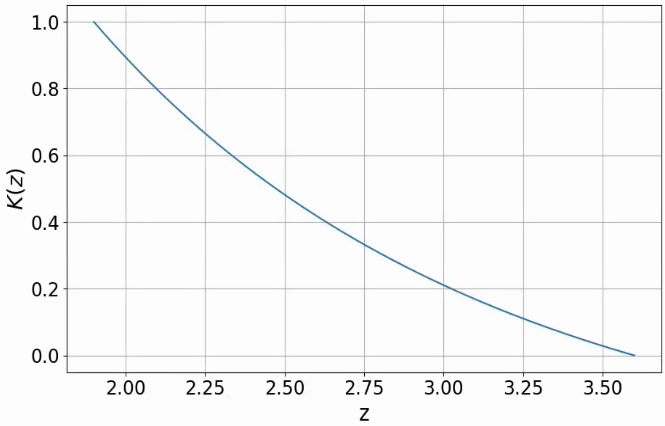
\includegraphics[scale=0.4]{kz}
  \caption{Coefficient $K(z)$ défini dans l'équation~\ref{eq:lognormal_interp}.}
\end{figure}
Les quasars sont ensuite tirés dans chaque voxcell, avec une probabilité $P \propto \hat \delta_{\textsc{QSO}}$. Pour ce faire, nous générons une variable $\phi$ aléatoire uniforme entre 0 et 1 dans chaque cellule. Les voxcells pour lesquelles $\phi < N(z) \hat \delta_{\textsc{QSO}}$ hébergent potentiellement un quasar. Le facteur $N(z)$ est un facteur de normalisation. Les quasars dont le redshift est en dehors de l'intervalle $[\num{1.8}; \num{3.6}]$ sont écartés.
% Les quasars dont l'ascension droite est en dehors de l'inverval $[ - \Delta \alpha ; \Delta \alpha]$ et dont la déclinaison est en dehors de l'inverval $[ - \Delta \delta ; \Delta \delta]$ sont aussi écartés.
Les quasars dont l'ascension droite et la déclinaison sont en dehors des intervalles $[ - \Delta \alpha ; \Delta \alpha]$ et $[ - \Delta \delta ; \Delta \delta]$ sont aussi écartés.
L'ascension droite $\alpha$ et la déclinaison $\delta$ du point $(\textsc{x},\textsc{y},\textsc{z})$ sont définies comme
\begin{align}
  \label{eq:radec}
  \alpha &= \arctan(\frac{
  \cos(\alpha_0)\textsc{x} - \sin(\delta_0)\sin(\alpha_0)\textsc{y} + \cos(\delta_0)\sin(\alpha_0)\textsc{z}
  }{
  - \sin(\alpha_0)\textsc{x} - \sin(\delta_0)\cos(\alpha_0)\textsc{y} + \cos(\delta_0)\cos(\alpha_0)\textsc{z}
           }) \; ,\\
  \delta &= \arcsin(\frac{
           \cos(\delta_0)\textsc{y} + \sin(\delta_0) \textsc{z}
           }{
           \sqrt{\textsc{x}^2 + \textsc{y}^2 + \textsc{z}^2}
           }) \; .
\end{align}
\textbf{Enfin, grâce au facteur de normalisation $N(z)$, les quasars sont tirés selon la distribution en $z$ normalisée prédite pour DESI. Cette distribution est présentée sur la figure~\ref{fig:dndz_qso}. Cependant, nous dirons environ deux fois plus de quasars, afin de pouvoir simuler, entre autre, la sélection des cibles à l'aide du code \texttt{quickquasars} (présenté dans la section~\ref{prov}).}
A la fin, nous obtenons environ \num{100} quasars à $z > \num{2.1}$ par degré carré.
\begin{figure}
  \centering
  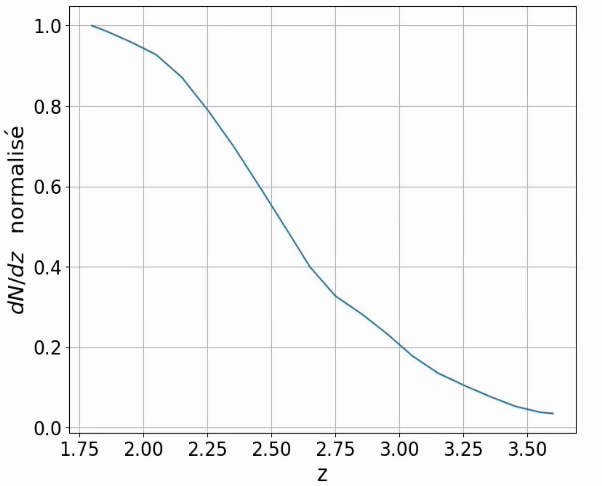
\includegraphics[scale=0.5]{dndz_qso}
  \caption{Distribution normalisée en redshift des quasars tirés dans les mocks.}
\end{figure}

\paragraph{}
Une fois les quasars tirés, nous les déplaçons proportionnellement à leur vitesse $v_{\parallel}$ le long de la ligne de visée. Celle ci est définie comme
\begin{equation}
  v_{\parallel} = \frac{v_{\textsc{x}} \textsc{x} + v_{\textsc{y}} \textsc{y} + v_{\textsc{z}} \textsc{z}}{\sqrt{\textsc{x}^2 + \textsc{y}^2 + \textsc{z}^2}} \; .
\end{equation}
\textbf{Ainsi, un quasar situé à une distance $R$ sera replacé le long de la ligne de visé à une distance
\begin{equation}
 R \rightarrow  R + \frac{1}{H(z)} v_{\parallel}(z) \; ,  % (1+z) \frac{dG}{dz} \frac{1}{H_0 \frac{dG}{dz}(z=0)} v_{\parallel} \; ,
\end{equation}
avec
\begin{equation}
 v_{\parallel}(z) = (1+z) \frac{dG}{dz} \frac{H(z)}{H_0 \frac{dG}{dz}(z=0)} v_{\parallel} \; .
\end{equation}
Le facteur $(1+z)$ vient de la conversion des distances en distances comobiles. Une fois tous les quasars déplacés, leur redshift est recalculé, puis ils sont stockés dans un catalogue. Pour chaque quasar, le catalogue contient leur position dans le ciel $(\alpha, \delta)$, leur redshift avec et sans RSD, ainsi qu'un identifiant unique.}


\subsection{Création des lignes de visée}
\label{subsec:los_interp}
A cette étape, nous disposons d'un catalogue de quasars, corrélé avec le champ de densité $\delta_{matière}$ qui sera utilisé pour construire l'absorption \lya{}. Nous pouvons donc créer les lignes de visées à partir de chaque quasar, et interpoler la boîte contenant le champ de densité, le long de ces lignes de visée.
Dans un premier temps, nous commençons par créer le vecteur en longueurs d'onde observées, sur lequel sera interpolé la boîte de densité. Nous choisissons une taille de pixel $d_{pix} = \SI{0.2}{\perh\Mpc}$. Les limites $\num{1.8} < z < \num{3.6}$ en redshift se traduisent par des limites\footnote{Ces limites sont aussi choisies afin de garantir un nombre entier de pixels.} $\num{3403.876} < \lambda < \SI{5592.082}{\angstrom}$ sur la longueur d'onde observée pour le \lya{}. Nous ajoutons la limite basse des spectrographes de DESI : $\lambda_{min} = \SI{3530}{\angstrom}$, que nous réduisons afin d'inclure certains métaux dans les forêts (voir ~\ref{prov}). Les longueurs d'onde observées couvrent donc $\num{3476.1877} < \lambda < \SI{5591.566}{\angstrom}$ à l'aide de \num{6524} pixels.

Une fois ce vecteur en longueur d'onde obtenu, nous le positionnons dans les boîtes afin de construire la ligne de visée à partir de chaque quasar.
% pour chaque quasar, nous calculons la position $(X,Y,Z)$ de chaque pixel.
D'abord, le pixel $\lambda_{\textsc{QSO}} = (1+z_{\textsc{QSO}}) \lambda_{\mathrm{Ly}\alpha}$ est placé à la position $(\textsc{x}_{\textsc{QSO}}, \textsc{y}_{\textsc{QSO}}, \textsc{z}_{\textsc{QSO}})$ du quasar, et le vecteur est dirigé vers l'observateur. Puis, pour chaque pixel $i$ entre $\lambda_{min} = \num{3476.1877}$ et $\lambda_{\textsc{QSO}}$, la position $(\textsc{x}_i, \textsc{y}_i, \textsc{z}_i)$ du pixel est déterminée.
% La boîte est alors interpolé puis lissé.
\textbf{Une moyenne pondérée avec un lissage gaussien est alors appliquée à la boîte.
Ce lissage est nécessaire afin d'éviter le crénelage (\emph{aliasing}) aux petites échelles.
  Nous choisissons un lissage de largeur $\sigma = d_{cell}$.
Pour chaque pixel, nous considérons les voxcells appartenant au cube de 7 voxcells de côté, centré sur le voxcell dans lequel se trouve le pixel. Ce cube correspond à considérer les voxcells compris à $\pm 3 \sigma$ du voxcell central. %, avec $\sigma = d_{cell}$ (\#prov validé par le plot, demander à JM).
Ceci représente donc, pour chaque pixel, une moyenne de \num{343} voxcells.
La figure~\ref{fig:smoothing11} présente la forêt \lya{} obtenue en considérant les voxcells à $\pm 1 \sigma$. Trop peu de voxcells sont considérés pour le calcul de chaque pixel, et la forêt obtenue contient des discontinuités. La figure~\ref{fig:smoothing23} présente la forêt obtenue en considérant les voxcells à $\pm 2 \sigma$ (orange) et $\pm 3 \sigma$ (bleu). La différence entre les deux est faible, cependant certaines discontinuités subsistent pour la forêt calculée avec $2 \sigma$, comme le montre le zoom sur le graphique de droite. Enfin, nous avons vérifié que les différences entre les forêts obtenues avec $3$ et $4 \sigma$ restent faibles. Nous nous limitons donc aux voxcells compris à $\pm 3 \sigma$ du voxcell central pour limiter le temps CPU.}
\begin{figure}
  \centering
  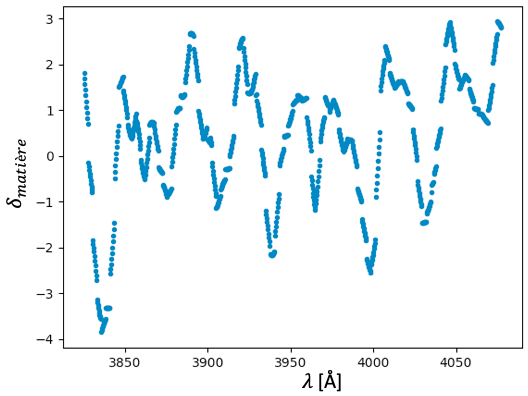
\includegraphics[scale=0.5]{smoothing11}
  \caption{bla}
  \label{fig:smoothing11}
\end{figure}
\begin{figure}
  \centering
  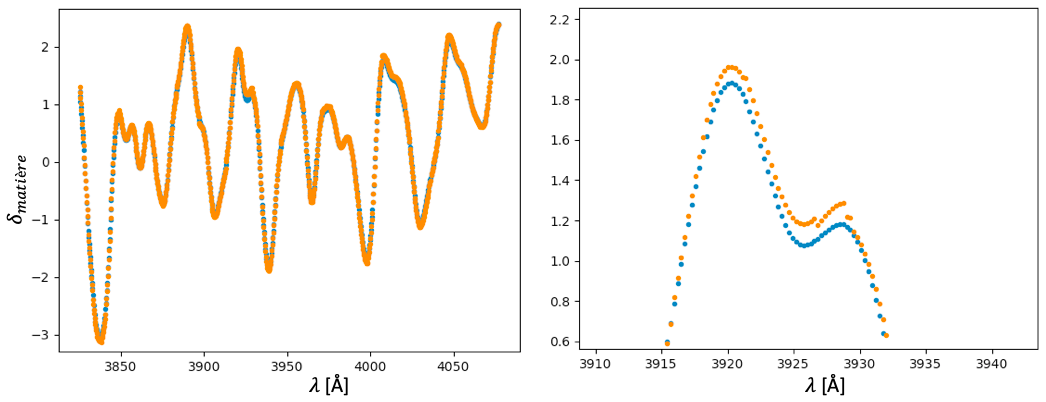
\includegraphics[scale=0.4]{smoothing23}
  \caption{bla}
  \label{fig:smoothing23}
\end{figure}
\textbf{Le pixel $i$ est donc donné par
% \begin{equation}
%   \delta_i = \sum_{j=0}^{342}  \frac{\delta(\vec r_j) \mathrm{e}^{\frac{-(\vec r_j - \vec r_i)^2 }{ \sigma_j^2}}}{\sigma_j^2} \; ,
% \end{equation}
% \#prov c'est pas correcte (voir le code)
\begin{equation}
  \delta_i = \frac{
    \sum_{j=0}^{342} \delta(\vec r_j) w_{ij}
  }{
    \sum_{j=0}^{342} w_{ij}
  } \; ,
\end{equation}
(\#prov c'est pas beau les limites des sommes qui sont pas au dessus/en dessous)
avec
\begin{equation}
  w_{ij} = \exp(\frac{
    -(\vec r_j - \vec r_i)^2
  }{
    \sigma^2
  }) \; ,
\end{equation}
où $\vec r_j$ est la position du voxcell $j$, $\vec r_i$ celle du pixel $i$, $\delta$ est la boîte à interpoler.
% , et enfin $\sigma^2 = d_{cell}^2$ est la largeur du lissage gaussien appliqué.
}
Ce calcul est effectué pour tous les pixels qui vérifient $\lambda_i < \lambda_{\textsc{QSO}}$, pour chaque quasar. Les boîtes interpolées sont la boîte $\delta_{matière}$ utilisée pour construire l'absorption \lya{}, les trois boîtes de vitesse utilisées pour ajouter les RSD aux HCD tirés dans chaque ligne de visée (voir section~\ref{subsec:hcd}), et les six boîtes de gradient de vitesse afin d'ajouter les RSD au champ \lya{}.


\subsection{De la densité à l'absorption}
Une fois les lignes de visés interpolées, nous pouvons transformer le champ de densité en absorption \lya{}. Ceci est fait via la formule FGPA :
\begin{equation}
  \label{eq:fgpa2}
F = \exp( - a(z) \mathrm{e}^{b(z) G(z) \delta_{matière}}) \;.  
\end{equation}

\subsubsection{Les petites échelles}
La boîte $\delta_{matière}$, utilisée dans l'équation~\ref{eq:fgpa2}, contient le champ de matière à grand échelle. Elle est construite grâce à la transformation de Fourier de la boîte $\delta_k$.
Cependant, ce champ est construit sur une grille de taille $d_{cell} = \SI{2.19}{\perh\Mpc}$. Par conséquent, la plus petite échelle accessible est
\begin{equation}
  k_N = \frac{2 \pi}{d_{cell}} \sim \SI{2.87}{\h\per\Mpc} \; .
\end{equation}
  Nous manquons donc toutes les fluctuations pour lesquelles $k > k_N$. Sans ces fluctuations le spectre de puissance à une dimension, défini comme
\begin{equation}
  \label{eq:p1d}
  P^{1D}(\kpar{}) = \frac{1}{2 \pi} \int_{\kpar{}}^{\infty} k P(k) dk \; ,
\end{equation}
ne possède pas la bonne amplitude. De plus, ce sont ces fluctuations aux petites échelles qui contribuent principalement à la variance du champ. Le champ $F$ construit ne possède donc pas le bon niveau de bruit.
Pour palier ce problème, nous rajoutons indépendamment sur chaque ligne de visée un champ $\delta_s$ (\emph{small scales} : petites échelles) au champ $\delta_{matière}$ que nous appelons désormais $\delta_{l}$ (\emph{large scales} : grandes échelles) :
\begin{equation}
  \label{eq:fgpa3}
  F = \exp( - a(z) \mathrm{e}^{b(z) G(z) (\delta_l + \delta_s)}) ;.
\end{equation}
Du fait que ce champ ne soit pas corrélé d'une ligne de visée à une autre, il ne participe pas à la fonction de corrélation à trois dimensions\footnote{Lors du calcul de la fonction de corrélation à 3 dimensions, nous ne considérons pas les paires de pixels issues de la même forêt (voir~\ref{prov})}. Afin d'ajouter la bonne quantité de fluctuations aux petites échelles, pour chaque ligne de visée nous générons un GRF à une dimension $\delta_{k,s}$, de la taille de la forêt. Puis, nous multiplions $\delta_{k,s}$ par
\begin{equation}
  \sqrt{\frac{P_{miss}(k)}{d_{pix}}} \; ,
\end{equation}
où $P_{miss}$ est le spectre de puissance qu'il faut appliquer à $\delta_{k,s}$ afin que $F$ possède le bon $P^{1D}$. Le calcul de $P_{miss}$ est détaillé dans la section~\ref{prov}. Enfin, nous obtenons $\delta_s$ à l'aide de la transformation de Fourier de $\delta_{k,s}$.

\subsubsection{Les RSD}
\label{subsubsec:rsdlya}
Une fois les petites échelles ajoutées, nous obtenons un champ d'absorption $F$ qui possède le bon spectre de puissance à 3 dimension pour les échelles $k_N < k < k_{max}$, avec
\begin{equation}
  k_{max} = \frac{2 \pi}{1536 d_{cell}} \sim \SI{1.9e-3}{\h\per\Mpc} \; ,
\end{equation}
ainsi que le bon spectre de puissance à une dimension.
Cependant, le champ d'absorption $F$ ne possède pas de RSD pour l'instant, car il est construit à partir du spectre de puissance $P_{matière}(k)$ qui est isotrope. Initiallement, nous pensions ajouster les RSD au niveau du spectre de puissance : multiplier le GRF intial par $(1 + \beta \mu^2)P_{matière}(k, \mu)$, avec $\mu = k_z / k$. Cependant, du fait que les lignes de visées ne sont pas parrallèles (elles l'étaient pour les mocks précédents, développés pour BOSS), nous ne pouvons pas confondre l'axe $k_z$ avec l'axe de la ligne de visée $\kpar{}$. Nous avons alors choisi d'utilisé le champ de gradient de vitesse $\eta_{\parallel}$, présenté dans la section~\ref{subsubsec:vitesses}. Plusieurs essais (\#prov les détailler ?)  ont été menés afin de savoir comment inclure correctement le champ $\eta_{\parallel}$ dans FGPA. Nous présentons dans les lignes qui suivent la solution retenue.
Le champ $\eta_{\parallel}$ est ajouté, en plus du champ $\delta_s$, au champ $\delta_l$. Ceci nous permet de retrouver la formule de Kaiser (équation~\ref{eq:kaiser5}). Afin de gérer la quantité de RSD, nous ajoutons un coefficient $c$, qui dépend de $z$. L'ajustement de ce paramètre nous permet d'obtenir la bonne dépendance en $z$ pour $\beta_{\mathrm{Ly}\alpha}$. La formule FGPA devient donc
\begin{equation}
  \label{eq:fgpa4}
  F = \exp( - a(z) \mathrm{e}^{b(z) G(z) (\delta_l + \delta_s + c(z)\eta_{\parallel})}) ;.  
\end{equation}
Les champs $\delta_l$, $\delta_s$ et $\eta_{\parallel}$ sont calculés à $z=0$, la dépendance en z étant prise en compte par le facteur $G(z)$. De plus, le facteur $f$ que nous avons laissé de cotê dans la section~\ref{subsubsec:vitesses} n'est pas explicité ici : pour les redshifts $z > 2$, l'univers est dominé par la matière et donc, en bonne approximation, nous avons $f(z) \sim 1$. Les paramètres $a(z)$, $b(z)$, $c(z)$, ainsi que $P_{miss}(z)$ sont ajustés afin d'obtenir le bon $b_{\mathrm{Ly}\alpha}(z)$, $\beta_{\mathrm{Ly}\alpha}(z)$, $\overline F(z)$ et $P^{1D}_{\mathrm{Ly}\alpha}(z)$. L'ajustement est décrit dans la section~\ref{prov}.

\subsubsection{La prédiction}
Il aurait été possible d'implémenter les RSD différemment. Une solution serait, par exemple, de déplacer chaque pixel d'absorption proportionnellement à la vitesse particulière du gaz dans la cellule considéré, puis de modifier l'absorption en fonction de gradient de vitesse dans cette cellule. En effet, si le gradient de vitesse est non nul, le gaz se retrouve comprimé par endroit, et détendu dans d'autres, modifiant l'absorption dans chaque cellule. Cette méthode pour ajouter les RSD dans des mocks \lya{} est la méthode choisie par \citet{Farr2019}.
% Ce n'est pas la méthode que nous choisissons ici, car celle-ci ne permet pas de prédire la fonction de corrélation obtenue avec les mocks. Dans le cas où $F$ est relié au GRF $\delta$ par une fonction analytique (équation~\ref{eq:fgpa4}), il est possible de relier la fonction de corrélation $\xi_F$ du champ $F$ à la fonction de corrélation $\xi_g$ du champ $\delta$ \citep{Font-Ribera2012}. Ces deux fonctions de corrélations sont reliées par la relation
La méthode que nous utilisons, décrite dans la section précédente, a l'avantage d'avoir une fonction de corrélation prédictible. C'est pour cela que nous avons fait le choix de cette méthode. Dans les lignes qui suivent, nous expliquons comment calculer la prédiction de la fonction de corrélation. Comme décrit par \citet{Font-Ribera2012}, il est possible de relier la fonction de correlation $\xi_F$ du champ $F$ à la fonction de corrélation $\xi_g$ du champ $\delta_g$. Ces deux fonctions de corrélations sont reliées par
\begin{equation}
  \label{eq:xig2xif}
  \xi_F(r_{12}) = \int_{- \infty}^{\infty} d\delta_{g1} \int_{- \infty}^{\infty} d\delta_{g2}
  \frac{
    \exp\left[-
      \frac{
        \delta_{g1}^2 + \delta_{g2}^2 - 2 \delta_{g1} \delta_{g2} \xi_g(r_{12})
      }{
        2 ( 1 - \xi_g^2(r_{12})))
      }\right]
  }{
    2 \pi \sqrt{1 - \xi_g^2(r_{12})}
  }
  \delta_F(\delta_{g1})\delta_F(\delta_{g2})
  \; ,
\end{equation}
où $\delta_g$ est un GRF de variance $1$, $\delta_F$ est le champ d'absorption calculé à partir du champ gaussien, et $r_{12}$ est la distance qui sépare les deux points où sont évalués les champs $\delta_g$ et $\delta_F$. Dans notre cas, le champ $\delta_g$ représente le champ $G(z)(\delta_l + \delta_c + c(z)\eta_{\parallel})$. Ce champ est un champ gaussien, de valeur moyenne nulle et de variance $\sigma_g^2$. Nous compensons le fait que $\sigma_g^2 \neq 1$ en remplaçant $\xi_g$ par $\xi_g / \sigma_g^2$ dans l'équation précédente. % Ainsi, grâce à l'équation~\ref{eq:xig2xif}, pour chaque valeur de $\xi_g \in [-1 ; 1]$, nous pouvons déterminer $\xi_F$.
L'équation~\ref{eq:xig2xif} ne dépendant que de la valeur de $\xi_g$, nous construisons une table qui permet de relier chaque valeur de $\xi_g \in [-1 ; 1]$ à la valeur $\xi_F$ correspondante.
% Afin d'obtenir la prédiction pour $\xi(r, \mu)$, nous utilisons les formules décrites dans \citet{hamilton_measuring_1992} :
% Afin d'obtenir la prédiction dans l'espace des redshifts, nous commençons par relier $\xi_g(r, \mu)$ à la fonction de corrélation $\xi(r)$ que suit le champ $\delta_l$ :
De plus, nous pouvons relier la fonction de corrélation dans l'espace des redshifts $\xi_g(r, \mu)$, à la fonction de corrélation $\xi(r)$ que suit le champ $\delta_l$ :
\begin{equation}
  \label{eq:hamilton1}
  \xi(r, \mu) = \xi_0(r) + \frac{1}{2}\left(3 \mu^2 - 1\right) \xi_2(r) + \frac{1}{8}\left(35 \mu^4 - 30 \mu^2 + 3\right) \xi_4(r) \; ,
\end{equation}
avec
\begin{align}
  \label{eq:hamilton2}
  \xi_0(r) &= \left(1 + \frac{2}{3} f + \frac{1}{5} f^2\right) \xi(r) \; , \\
  \xi_2(r) &= \left(\frac{4}{3} f + \frac{4}{7} f^2\right) \left[\xi(r) - \overline \xi(r)\right] \; , \\
  \xi_4(r) &= \frac{8}{35} f^2\left[\xi(r) + \frac{5}{2} \overline \xi(r) - \frac{7}{2} \overline{\overline \xi}(r)\right] \; ,
\end{align}
et
\begin{align}
  \label{eq:hamilton3}
  \overline \xi(r) = 3 r^{-3} \int_0^r \xi(s) s^2 ds \; , \\
  \overline{\overline \xi}(r) = 5 r^{-5} \int_0^r \xi(s) s^4 ds \; .
\end{align}
Ces équations sont décrites dans \citet{hamilton_measuring_1992}.
Afin d'obtenir la prédiction $\xi_F^{pred}(r, \mu)$, nous commençons par calculer  le spectre de puissance que suit la boîte $\delta_l$ :
\begin{equation}
  P(k) = W^2(k)P_{matière}(z=0) \; ,
\end{equation}
où $W$ est le terme représentant le lissage gaussien appliqué à la boîte $\delta_l$ (voir section~\ref{subsec:los_interp}) :
\begin{equation}
  W(k) = \mathrm{e}^{- \frac{k^2 d_{cell}^2}{2}} \;.
\end{equation}
(\#prov il y a pas un facteur $\frac{1}{2}$ en trop ? on a $\sigma_{smooth}^2 = 2 d_{cell}^2$)

A l'aide d'une transformation de Fourier, nous obtenons la fonction de corrélation $\xi(r)$ que suit la boîte interpolée $\delta_l$.
% Nous définissons le champ $\delta_g$ comme
% \begin{equation}
%   \delta_g = G(z)(\delta_l + \delta_c + c(z)\eta_{\parallel}) \; .
% \end{equation}
Puis, nous calculons la fonction de corrélation dans l'espace des redshifts $\xi_g(r, \mu)$ que suit le champ $\delta_g$ gràce à l'équation~\ref{eq:hamilton1}. Enfin, pour tous les couples $(r,\mu)$ nécessaires, nous obtenons la fonction de corrélation $\xi_F(r, \mu)$ du champ $F$ comme la valeur correspondante à la valeur tabulée $\xi_g(r, \mu) / \sigma_g^2$ pour $\xi_g$.
(\#prov un plot de la prédiction ?)


\subsection{Ajout des HCD}
\label{subsec:hcd}
Les HCD ont un effet important dans les fonctions de corrélation, nous simulons donc aussi leur présence. De manière à avoir une corrélation entre les HCD et les autres traceurs des mocks, nous utilisons la boîte de densité $\delta_l$ pour tirer les HCD. Nous ne considérons pas la somme $\delta_l + \delta_s$ car les HCD sont des surdensités à grandes échelles : une résolution de \SI{2.19}{\perh\Mpc} est suffisante. De plus, l'ajout de $\delta_s$ bruiterait la corrélation entre les HCD et les autres traceurs.

% Nous commençons donc avec le champ de densité $\delta_l$ interpolé le long de la ligne de visée. Pour chaque ligne de visée,
Contrairement aux quasars, les HCD sont tirés proportionnellement au champ $\delta_l$. Nous identifions les cellules dans lesquelles $\delta_l$ est au dessus d'un certain seuil, puis les HCD sont tirés dans ces cellules selon une loi de Poisson. Le seuil $\nu$ est défini en fonction du biais souhaité pour les HCD. Pour un seuil $\nu$, le biais obtenu est donné par
\begin{equation}
  b_{\nu} = \frac{pdf(\nu)}{cdf(-\nu)} \; ,
\end{equation}
où $pdf(\nu)$ donne la densité de probabilité de $\nu$, et $cdf(-\nu)$ est la fonction de répartition : la probabilité d'être au dessus du seuil $\nu$. Ainsi, pour avoir un biais de 2, il faut que la probabilité que le champ prenne la valeur $\nu$ soit 2 fois plus grande que la probabilité que le champ soit au dessus du seuil $\nu$. Afin d'obtenir le seuil pour un biais donné, nous calculons $b_{\nu}$ pour une large gamme de seuils $\nu$ puis nous interpolons $b_{\nu}$ sur $\nu$. Ainsi, pour un biais $b$, nous connaissons le seuil $\nu(b)$ à choisir.
Dans notre cas, le champ $\delta_l$ suit une densité de probabilité gaussienne. Cependant, sa variance n'est pas égale à 1. De plus, le champ $\delta_l$ interpolé le long des lignes de visée correspond au champ de matière à $z=0$. Ainsi, pour obtenir un biais $b_{\textsc{HCD}}$, pour chaque redshift nous  calculons le seuil $\nu$ comme si nous visions un biais $b = b_{\textsc{HCD}} \sigma_l G(z)$. Le terme $\sigma_l$ prend en compte la variance du champ $\delta_l$, et $G(z)$ le fait que $\delta_l$ soit construit à $z=0$.
Une fois les cellules pouvant héberger un HCD identifiées, nous tirons dans chacune d'entre elles les HCD avec une loi de poisson de paramètre
\begin{equation}
  \lambda(z) = \frac{N(z)}{cdf(-\nu(z))} \; ,
\end{equation}
où $N(z)$ donne le nombre moyen de HCD attendu par cellule et $\nu(z)$ le seuil au redshift $z$. Le nombre de HCD attendu est donné par la librairie \texttt{pyigm}\footnote{https://github.com/pyigm}. La distribution en redshift des HCD est présenté sur le graphique de gauche de la figure~\ref{fig:distrib_dla}. Une fois tous les HCD tirés, nous leur assignons une densité de colonne dans la gamme $\num{17.2} < \log(n_{HI}) < \num{22.5}$, selon la distribution donnée par \texttt{pyigm}. Cette distribution est présentée sur le graphique de droite de la figure~\ref{fig:distrib_dla}.
\begin{figure}
  \centering
  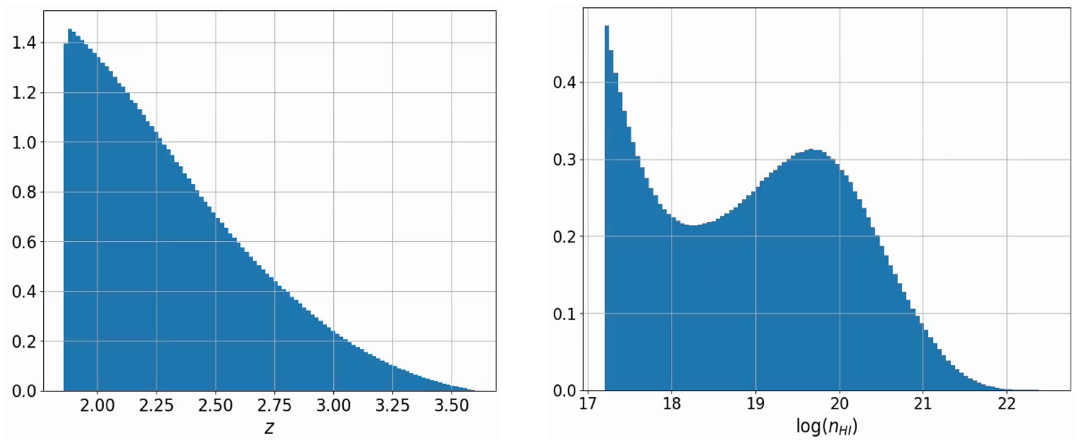
\includegraphics[scale=0.38]{distrib_dla}
  \caption{Gauche : distribution normalisée en redshift des HCD. Droite : distribution normalisée de $\log(n_{HI})$ des HCD. Ces distributions proviennent de la librairie \texttt{pyigm}.}
  \label{fig:distrib_dla}
\end{figure}
Enfin, nous ajoutons les RSD aux HCD tirés. Chaque HCD tiré est déplacé le long de la ligne de visée proportionnellement à la vitesse
\begin{equation}
v_{\parallel} = \frac{v_{\textsc{x}} \textsc{x} + v_{\textsc{y}} \textsc{y} + v_{\textsc{z}} \textsc{z}}{\sqrt{\textsc{x}^2 + \textsc{y}^2 + \textsc{z}^2}} \; ,
\end{equation}
où $v_{\textsc{x}}$, $v_{\textsc{y}}$ et $v_{\textsc{z}}$ sont les boîtes de vitesse interpolées le long de la ligne de visée. Ainsi, un HCD à un redshift $z$ sera déplacé à un redshift
\begin{equation}
   z \rightarrow  z + (1+z) H(z) \frac{dG}{dz} \frac{1}{H_0 \frac{dG}{dz}(z=0)} v_{\parallel} \; .
\end{equation}
Dans les mocks que nous décrivons ici, le profil d'absorption des HCD n'est pas ajouté dans les forêts. Nous produisons uniquement un catalogue qui regroupe tous les HCD tirés. Le profile d'absorption est ajouté au spectre de chaque quasar par le code \texttt{quickquasars}, qui utilise le catalogue de HCD que nous produisons.


\section{Production des mocks}
Comme expliqué au début de ce chapitre, l'objectif des mocks est de reproduire les données d'eBOSS et de DESI. Etant donné que le relevé d'eBOSS est contenu dans le relevé de DESI, nous simulons directement le relevé DESI. Ainsi, lorsque nous avons besoin de simuler le relevé d'eBOSS, nous retirons les quasars qui ne sont pas contenu dans ce relevé. La taille des boîtes choisie ($\num{2560}\times\num{2560}\times\num{1536}$ voxcells) et leur résolution (\SI{2.19}{\perh\Mpc}) ne suffisent pas à couvrir les \num{14000} degrés carrés de DESI. Pour palier ce problème, nous construisons sept \emph{chunks} indépendants, que nous assemblons pour former le relevé de DESI. Le découpage du relevé en sept chunks est montré sur la figure~\ref{prov} (\#prov faire une figure). Ce choix d'assembler sept boîtes de densité plutôt que d'en utiliser une seule a été contraint par la mémoire maximale des noeuds. Les mocks ont été produit grâce au centre de calcul NERSC\footnote{National Energy Research Scientific Computing Center (NERSC), a U.S. Department of Energy Office of Science User Facility operated under Contract No. DE-AC02-05CH11231.}, avec la machine Cori. Sur cette machine, nous avons utilisé les noeuds ``Haswell'', au nombre de \num{2388}. Chaque noeud possède 32 c{\oe}urs, chacun possèdant 2 hyper-threads. Chaque noeud peut donc gérer 64 tâches simultanément. De plus, ces noeuds possèdent $\num{128}\,\mathrm{Go}$ de mémoire vive. De manière à créer nos boîtes de densité, via la transformation de Fourier à trois dimensions, il faut, pour chaque boîte, que l'intégralité de son contenu soit accessible depuis un même endroit. Nous pourrions distribuer la mémoire et effectuer la transformation de Fourier sur plusieurs noeuds à l'aide de la librairie MPI. Cependant nous avons choisi de ne pas utiliser cette librairie et d'effectuer les transformations de Fourier sur un seul noeud, ce qui explique le découpage du relevé en sept chunks indépendants. Nous profitons néanmoins des 64 threads de chaque noeud pour paralléliser notre code.

Dans les lignes qui suivent, nous détaillons les différents éléments du code.
Le schéma~\ref{prov} résume la situation (\#prov faire le schéma).
Le première module, \texttt{interpolate\_pk.py} permet de calculer puis d'interpoler les quatres spectres de puissance $P_{\textsc{QSO},i}$ et $P_{matière}$ sur la grille $\num{2560}\times\num{2560}\times\num{1536}$. Le code est lancé séparément sur 16 morceaux de la boîte, puis le code \texttt{merge\_pk.py} permet de rassembler des 16 morceaux des spectres de puissance interpolés et de les sauver au format FITS (Flexible Image Transport System). Cette étape est effectuée une seule fois, car les spectres de puissance sont communs à toutes les réalisations. Le module suivant est \texttt{make\_boxes.py}. Ce code lit les spectres de puissance interpolés puis construit les différentes boîtes de densité, de vitesse et de gradient de vitesse décrits dans la section~\ref{subsec:densityfields}. Ce code est lancé sept fois, afin de produire les boîtes pour les septs chunks. Une fois toutes les boîtes produites, les quasars sont tirés (section~\ref{subsec:qso}) grâce au code \texttt{draw\_qso.py}. Afin d'accélerer la production des mocks, les boîtes sont partagées en \num{512} tranches selon l'axe \textsc{x}. Ces tranches, de taille $\num{5}\times\num{2560}\times\num{1536}$, sont traitées séparément. Ce code est donc tourné en parallèle \num{512} fois, sur 16 noeuds $\times$ 32 threads. Une fois les quasars tirés, les lignes de visée sont interpolées (section~\ref{subsec:los_interp}) avec le code \texttt{make\_spectra.py}. De la même manière que le code précédent, il tourne en parallèle \num{512} fois, sur 16 noeuds $\times$ 32 threads. Une fois tous les quasars traités, les morceaux de ligne de visée sont mis bout à bout grâce au code \texttt{merge\_spectra.py}. Encore une fois, le code tourne en parallèle \num{512} fois. Lorsque les lignes de visée sont reconstruites, la formule FGPA est appliquée afin d'obtenir le champ de transmission $F$ pour chaque ligne de visée.
La dernière étape consiste à regrouper le résultat de chaque chunk. Le module \texttt{merge\_qso.py} permet de lire tous les quasars tirés dans chaque tranche de chaque chunk et de créer un catalogue global appelé \texttt{master.fits}. Une fois le catalogue construit, le code \texttt{dla\_saclay.py} tire les HCD dans chaque ligne de visée. Le code est tourné sur les septs chunks en parallèle. Puis le module \texttt{merge\_dla.py}, comme pour les quasars, permet de regrouper tous les HCD tirés et de construire le catalogue global \texttt{master\_DLA.fits}. Enfin le code \texttt{make\_transmissions.py} permet de mettre les fichiers contenant les forêts au bon format : les forêts sont regroupées par HEALPix pixel (\#prov expliquer ou mettre une ref ?) et sont stockées dans les fichiers
\begin{equation*}
  \texttt{\textsc{n}/\textsc{pix}/transmission-nside-\textsc{pix}.fits.gz} \; ,
\end{equation*}
où $\texttt{nside} = \num{16}$ est la résolution du schéma HEALPix utilisé, \texttt{\textsc{pix}} donne le numéro du pixel HEALPix, et $\texttt{\textsc{n}}$ est le résultat de la division euclidienne de \texttt{\textsc{pix}} par \num{100}.
Cette dernière étape est effectuée sur un noeud, \texttt{make\_transmissions.py} étant lancé en parallèle sur 64 sous-échantillons des HEALPix pixels.


\paragraph{}
Pour les analyses \lya{} d'eBOSS et de DESI, nous avons décidé de produire \num{100} réalisations des mocks, afin d'avoir suffisamment de statistique pour étudier finement les potentielles systématiques. Nous avons organisé la production de ces 100 réalisations en deux étapes. Premièrement, nous avons effectué la \emph{pré-production}. Cette étape consiste à créer les boîtes contenant les différents GRF, puis à tirer les quasars et enfin reconstruire la densité, les vitesses et gradients de vitesse, le long de chaque ligne de visée. Ceci correspond aux codes \texttt{make\_boxes.py}, \texttt{draw\_qso.py} et \texttt{make\_spectra.ppy}. Cette étape est la plus coûteuse en temps de calcul : environ 43 heures CPU sur un noeud de Cori pour produire les septs chunks d'une réalisation. L'ensemble des fichiers temporaires propres à une réalisation pré-produite est estimé à $\sim 7 \times \num{550}\,\mathrm{Go}$ sur disque. Cependant, nous stockons uniquement les lignes de visée interpolées, et la boîte $\delta_k$, ce qui représente $\sim \num{340}\,\mathrm{Go}$ sur disque, par réalisation.

Une certain nombre de problèmes informatiques, liés au centre de calcul NERSC, ont ralenti la phase de pré-production. Le principal problème venait du temps de lecture et d'écriture, qui par moment pouvait être multiplié par un facteur cent. Plus de trentes secondes étaient parfois nécessaires pour accéder à un simple fichier. Ce problème a été identifié comme venant du transfert des \emph{meta data} sur le centre de calcul. Le code le plus affecté est \texttt{make\_boxes.py}, car il écrit énormément de fichiers différents, correspondant aux différents slices des boîtes, et destinés à être lus par les codes \texttt{draw\_qso.py} et \texttt{make\_spectra.py}. Pour palier ce problème, nous avons décidé d'essayer de faire tourner les codes sur les noeuds de Cori appelés \emph{Burst Buffer}. Ces noeuds possèdent des disques SSD (Solid-State drive), ce qui permet une lecture et une écriture très rapide. Une fois les codes exécutés, les données produites sont déplacées sur les disques durs habituels. Les noeuds Burst Buffer ont permis d'accélérer l'exécution du code \texttt{make\_boxes.py} par un facteur $\sim \num{2}$, passant d'environ deux heures à une heure seulement. Une vintaine de réalisation ont été produites en utilisant ces noeuds. Cependant, ils sont devenus instables au cours de la production. D'autre part, les problèmes liés aux transferts des meta data avaient été stabilisés entre temps. Nous sommes donc retournés à l'utilisation des noeuds classiques de Cori pour finir la production. Pour les 40 dernières réalisations, le temps d'exécution de \texttt{make\_boxes.py} variait entre trois et quatres heures.

% Celle-ci a nécessité environ six mois avant d'être complète.
% Ce temps nous a permis de choisir les paramètres \lya{} souhaités,
Le temps laissé par les six mois nécessaires à la production nous a permis de choisir les paramètres \lya{} souhaités,
et d'ajuster les paramètres de la formule FGPA (équation~\ref{eq:fgpa4}) en conséquence (voir section~\ref{prov}). Une fois ces paramètres ajustés et la phase de pré-production terminée, nous avons mené la phase de \emph{post-production}. Cette phase consiste à créer les spectres d'absorption à partir des densités interpolées le long des lignes de visée, puis à regrouper tous les fichiers de sortie afin de les mettre au format décrit précédemment. Cette étape est beaucoup plus rapide, elle prend l'équivalent d'environ 6 heures CPU sur un noeud de Cori. Une fois la production complète effectuée, la place sur disque d'une réalisation, sans compter les fichiers temporaires, correspond à environ $\num{15}\,\mathrm{Go}$ sur disque.




\bibliography{../source/library}
\end{document}
